Ghidra är ett avancerat verktyg som gör statisk analys bortom syftet med AMBA,
men AMBA har ett par likheter. Ghidra kan representera en kontrollflödesgraf
för en given binär på två olika sätt: \textit{Flow Graph} och \textit{Code Flow
    Graph}~\cite{ghidra_website}.

\begin{figure}[H]
    \begin{subfigure}{0.3\textwidth}
        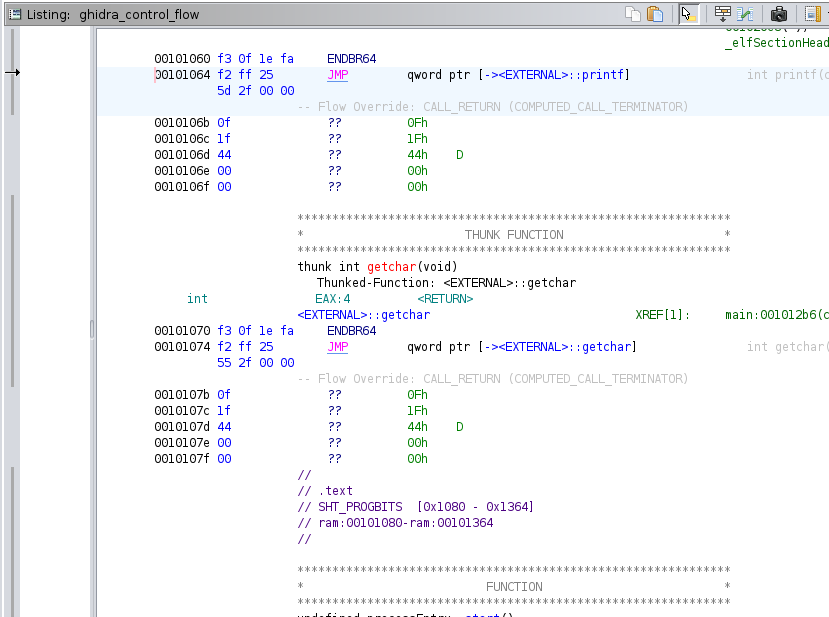
\includegraphics[width=\linewidth]{figures/ghidra_code_listing.png}
        \caption{Ghidras code listing.} \label{fig:ghidra_code_listing}
    \end{subfigure}
    \hspace*{\fill}
    \begin{subfigure}{0.3\textwidth}
        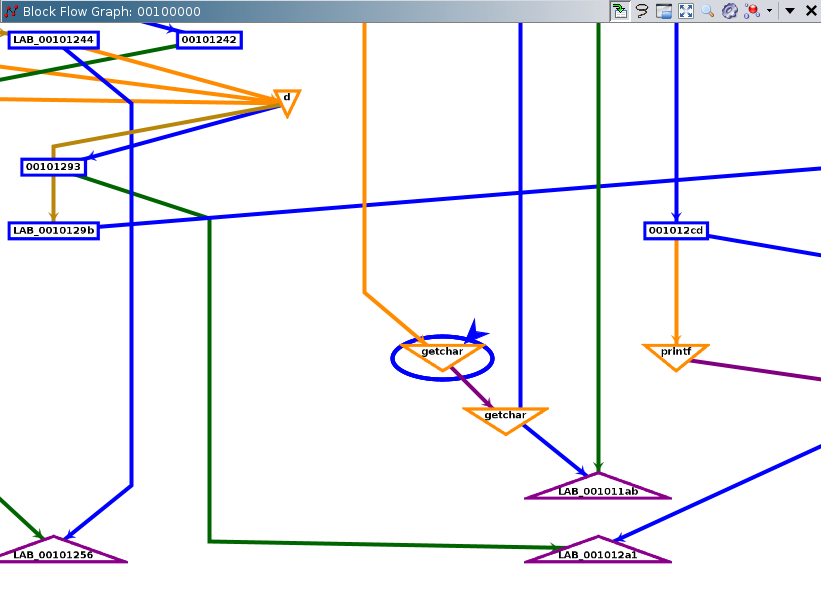
\includegraphics[width=\linewidth]{figures/ghidra_block_flow_graph.png}
        \caption{Ghidras block-flow-graph.}
        \label{fig:ghidra_block_graph}
    \end{subfigure}
    \hspace*{\fill}
    \begin{subfigure}{0.3\textwidth}
        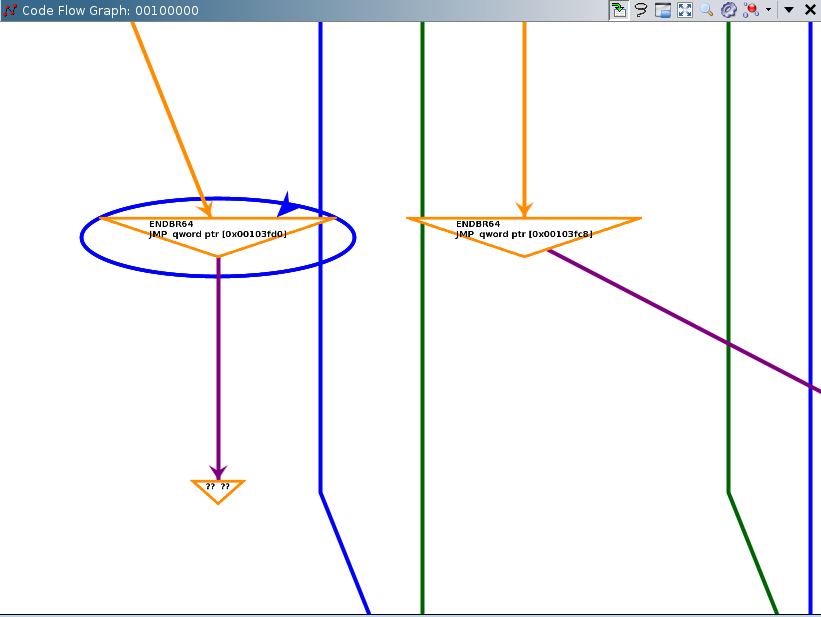
\includegraphics[width=\linewidth]{figures/ghidra_code_flow.png}
        \caption{Ghidras code-flow-graph.} \label{fig:ghidra_code_flow_graph}
    \end{subfigure}

    \caption{Tre primära vyer i verktyget Ghidra för att representera ett programs
        kontrollflödesgraf.} \label{fig:ghidra_figures}
\end{figure}

Ghidra kompletterar dessa vyer med en \textit{code listing}, en primär vy där
binärens disassemblerade kod listas. Användaren kan fritt välja att bilda en
graf från ett markerat \textit{code block}, vilket är Ghidras utökade
specifikation på ett \emph{basic block}, från Ghidras code
listing~\cite{ghidra_website}. AMBA har liknande funktionalitet, se
figur~\ref{fig:graf-basic}, och kan visualisera binärens fullständiga
disassemblerade kod för en given nod, om debugdata finns tillgänglig, men saknar
större kontext likt Ghidras code listing. En fördel mot Ghidras representation
är AMBAs fem olika sätt att representera en binärs kontrollflöde på: \textit{Raw
    Basic Block Graph}, \textit{Compressed Block Graph}, \textit{State Graph},
\textit{Merged Block Graph} och \textit{Compressed Merged Block Graph}.  Genom
att använda dessa fem olika vyer kan en användare bilda en större förståelse om
en given binär, dels genom att exempelvis visualisera alla symboliska tillstånd
som \stoe{} skapar i kombination med färgade noder som indikerar på starkt
kopplade komponenter (jfr.\ eng. \emph{strongly connected components}).

Kännedom om starkt kopplade komponenter i en kontrollflödesgraf är i synnerhet
intressant vid analys av binärer utan källkod, eftersom dessa delgrafer speglar
en starkare koppling mellan noderna och indikerar på en sektion i binären som
troligtvis har större relevans än en sektion som saknar eller har betydligt
färre starkt kopplade komponenter. Ett typiskt mönster man kan se med starkt
kopplade komponenter är icke-nestlade loopar.

\begin{figure}
    \centering
    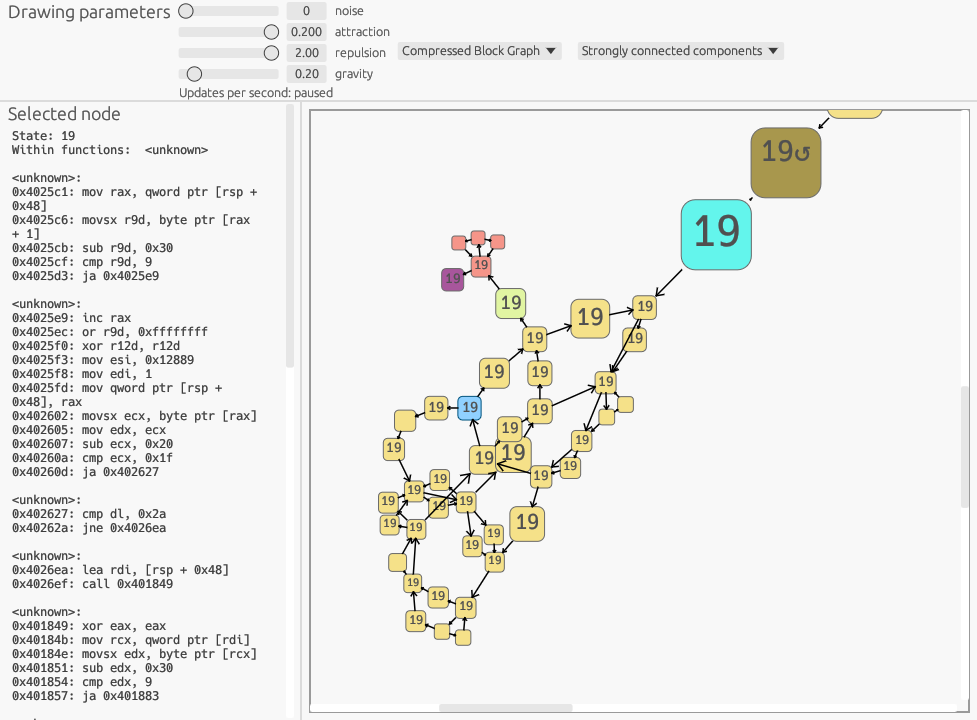
\includegraphics[width=0.7\textwidth]{figures/graph_scc.png}
    \caption{
        En del av AMBAs komprimerade basic-block-graf, färglagd efter starkt
        anslutna komponenter för testprogrammet control-flow
    }\label{fig:graf-scc}
\end{figure}

En användare skulle exempelvis kunna använda AMBAs nodfärgläggning för att bilda
en större uppfattning om en viss del i binären och sedan komplettera med
nodernas minnesaddresser för att visualisera samma sektion i ett mer avancerat
verktyg som Ghidra. Ett typiskt användningsfall skulle kunna vara att i Ghidra
söka efter strängar som ger mer information i den givna kodsektionen från AMBA
eller använda Ghidras analysmetoder för att dekompilera binärens instruktioner
till ett mer läsbart format i form av pseudokod.
